\section{Vektorer}
En vektor er et objekt defineret ved en retning og en længde, som kan repræsenteres som en matrix, der enten kun har én sølje eller én række.
Det vil sige, at en vektor er et særtilfælde af en matrix, og alle regneregler for matricer, gør sig derfor gældende for vektorer, men ikke alle regneregler for vektorer kan bruges for matricer.
En vektor med kun én søjle kaldes en søjlevektor, mens en vektor med kun én række kaldes en rækkevektor.
Vektorer anvendes blandt andet til at repræsentere rækker og søjler i matricer. 
I dette tilfælde er vektorerne derved delmatricer af den originale matrix.
Indgangene i en vektor kaldes vektorens vektorkomponenter, og vil være udgjort af vektorens koordinator.

\begin{defn}[Søjlevektor]
Lad $\underset{m \times n}{A}$ være en matrix, så vil en \textbf{søjlevektor} være en delmatrix med kun en søjle og alle søjlens rækkekomponenter
\begin{align*}
\vec{v}=\underset{m \times 1}{A} = 
\begin{bmatrix}
a_{1,i}\\
a_{2,i}\\
\vdots \\
a_{m-1,i}\\
a_{m,i} \\
\end{bmatrix},\qquad  i\in \{1,...,n\}
\end{align*}
Vektoren $\vec{v}$ siges at have dimension $m$ og tilhører  $\mathds{R}^m$.
\end{defn}

På samme måde kan en rækkevektor defineres


\begin{defn}[Rækkevektor]
Lad $\underset{m \times n}{A}$ være en matrix, så vil en \textbf{rækkevektor} være en delmatrix med kun en række og alle rækkens søjlekomponenter
%En \textbf{Række vektor} er en matrice med 1 række og n søjler
\begin{align*}
\underset{1 \times n}{A} = 
\rvect{a_{j,1} & a_{j,2} & \dots & a_{j,n-1} & a_{j,n}},
\qquad  j\in \{1,...,m\}
\end{align*}
Vektoren $\vec{v}$ siges at have dimension $n$ og tilhører $\mathds{R}^n$.
\end{defn}
Bemærk at hvis henholdsvis $m$ eller $n$ er $1$, så er matricen i forvejen en vektor.\\
\\
Ved addition af to vektorer, placeres vektorerne i samme begyndelsespunkt, så de udspænder to sider af et parallelogram. Da følger af parallelogram-loven, at diagonalen af det fulde parallelogram er summen af de to vektorer.
Repræsenteres  vektorene som en matrix, er summen af vektorene, en ny matrix, hvis $i$te indgang er summen af de to vektores $i$te indgange. 
Bemærk derfor, at det ikke er muligt at lægge to vektorer sammen af forskellig dimension. Det er heller ikke muligt at finde summen af en søjle- og rækkevektor, selvom de har samme dimension.

%Addition af to vektorer kan repræsenteres grafisk med pile, ved at tage to ikke-nul vektorer $\vec{u}$ og $\vec{v}$ og forme et parallelogram med vektorene som parallelogrammets sider. I følge parallelogram loven vil diagonalen af parallelogrammet være de to vektor lagt sammen $\vec{u}+\vec{v}$.
%Mangler firgur 1.3 fra lial bogen
\begin{defn}[Addition af to vektor]
Lad $\vec{v}, \vec{u}, \vec{w} \in \mathds{R}^n$, så $\vec{w}=\vec{u}+\vec{v}$, da er den $i$te indgang i $\vec{w}$ givet som $w_i = u_i + v_i$. 
%Lad $\underset{m \times 1}{A}$ og $\underset{m \times 1}{B}$ være to vektorer med samme størrelse. Da vil additionen af de to vektorer give en vektor, $\underset{m \times 1}{C}$, hvor hver komponent er summen af de tilsvarende komponenter i $\underset{m \times 1}{A}$ og $\underset{m \times 1}{B}$.
%\begin{align*}
%\underset{m \times 1}{A} = 
%\begin{bmatrix}
%a_{1,1}\\
%a_{2,1}\\
%\vdots \\
%a_{m-1,1}\\
%a_{m,1} \\
%\end{bmatrix}
%\qquad
%\underset{m \times 1}{B} = 
%\begin{bmatrix}
%b_{1,1}\\
%b_{2,1}\\
%\vdots \\
%b_{m-1,1}\\
%b_{m,1} \\
%\end{bmatrix}
%\end{align*} 
%\begin{align*}
%C=A+B=
%\begin{bmatrix}
%a_{1,1}\\
%a_{2,1}\\
%\vdots \\
%a_{m-1,1}\\
%a_{m,1} \\
%\end{bmatrix}
%+
%\begin{bmatrix}
%b_{1,1}\\
%b_{2,1}\\
%\vdots \\
%b_{m-1,1}\\
%b_{m,1} \\
%\end{bmatrix}
%=
%\begin{bmatrix}
%a_{1,1}+b_{1,1}\\
%a_{2,1}+b_{2,1}\\
%\vdots \\
%a_{m-1,1}+b_{m-1,1}\\
%a_{m,1}+b_{m,1} \\
%\end{bmatrix}
%\end{align*}
\end{defn}
\begin{eks}
Betragt de to $4$ dimensionelle vektorer
\begin{align*}
\vec{v}=
\begin{bmatrix}
4\\
1\\
0\\
-5\\
\end{bmatrix}
%\hspace{3cm}
\vec{u}=
\begin{bmatrix}
7\\
4\\
-2\\
-5\\
\end{bmatrix}
\end{align*}
Da er deres sum 
\begin{align*}
\vec{v}+\vec{u}=
\begin{bmatrix}
4\\
1\\
0\\
-5\\
\end{bmatrix}
+
\begin{bmatrix}
7\\
4\\
-2\\
-4\\
\end{bmatrix}
=
\begin{bmatrix}
4+7\\
1+4\\
0-2\\
-5-4\\
\end{bmatrix}
=
\begin{bmatrix}
11\\
5\\
-2\\
-9\\
\end{bmatrix}
\end{align*}
\end{eks}

Hvis en vektor kan lægges til en anden vektor, må det også være muligt at skalere den. Det vil sige multiplicere den med en konstant, eftersom $2\vec{v}=\vec{v}+\vec{v}$.\\ %giver god mening, men det lyder som et bevis
\begin{figure}[h]
\begin{center}
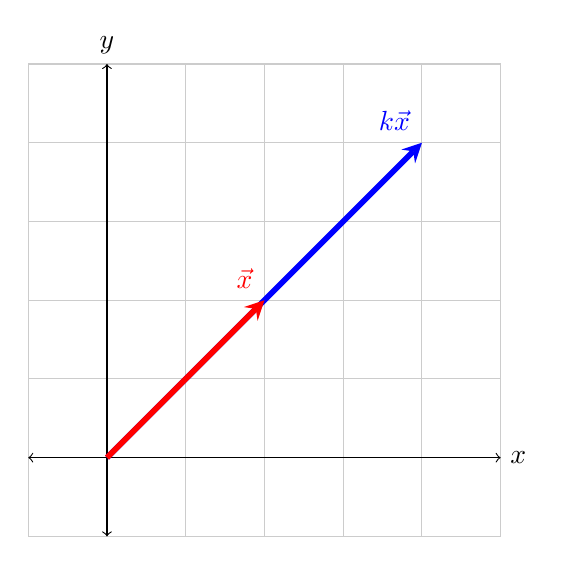
\begin{tikzpicture}
  \draw[thin,gray!40] (-1,-1) grid (5,5); %laver Grid
  \draw[<->] (-1,0)--(5,0) node[right]{$x$}; %x-aksen
  \draw[<->] (0,-1)--(0,5) node[above]{$y$}; %y-aksen
  \draw[line width=2pt,blue,-stealth](0,0)--(4,4) node[above left]{$k\vec{x}$}; %blå vektor
  \draw[line width=2pt,red,-stealth](0,0)--(2,2) node[above left]{$\vec{x}$}; %rød vektor
\end{tikzpicture}
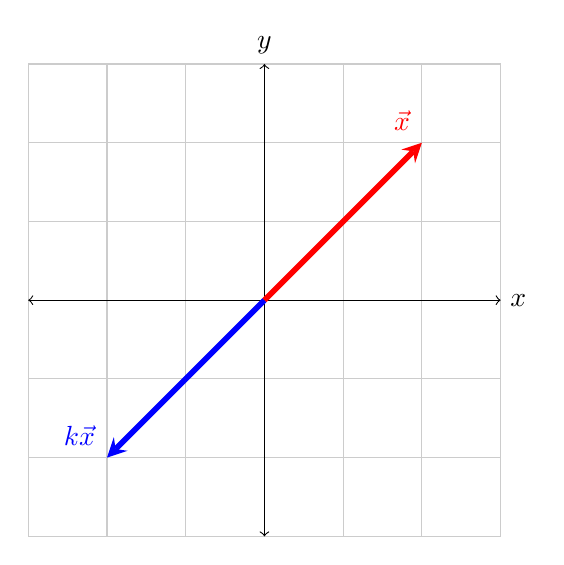
\begin{tikzpicture}
  \draw[thin,gray!40] (-3,-3) grid (3,3);
  \draw[<->] (-3,0)--(3,0) node[right]{$x$};
  \draw[<->] (0,-3)--(0,3) node[above]{$y$};
  \draw[line width=2pt,blue,-stealth](0,0)--(-2,-2) node[above left]{$k\vec{x}$};
  \draw[line width=2pt,red,-stealth](0,0)--(2,2) node[above left]{$\vec{x}$};
\end{tikzpicture}
\caption{Billede 1, viser skalar multiplikationen $k \cdot \vec{x}$, for $k=2$, mens $k=-1$ på billede 2}
\end{center}
\label{fig:vektorskalar}
\end{figure}
Derfor må den nye vektors komponenter være den originale vektors komponenter multipliceret med skalaren.
\begin{defn}[Vektor skalar]
Lad $\vec{v}, \vec{u}$ være en vektorer i $\mathds{R}^n$, og $k$ en skalar, så $\vec{u} = k \cdot \vec{v}$, da er den $i$te indgang i $\vec{u}$ givet ved $u_i = k\cdot v_i$.
% da er et \textbf{vektor skalar} produktet af den vektorens komponenter multipliceret med konstanten.
%da er et \textbf{vektor skalar } givet ved,
%En \textbf{Vektor skalar} er produktet af en vektor $\vec{x}$
%som bliver multipliceret med en konstant $k$ kaldet skalar. Denne vektor peger i samme retning, men har en anden længde.
%\begin{align*}
%\vec{x}=\begin{bmatrix}
%%x_1\\
%%x_2\\
%%\vdots\\
%%x_{n-1}\\
%%x_n
%%\end{bmatrix}\\
%k\vec{x}=k\begin{bmatrix}
%x_1\\
%x_2\\
%\vdots\\
%x_{n-1}\\
%\end{bmatrix}=
%\begin{bmatrix}
%kx_1\\
%kx_2\\
%\vdots\\
%kx_{n-1}\\
%kx_n\\
%\end{bmatrix}
%\end{align*}
\end{defn}
\begin{eks}
En vektor $\vec{x}$ med komponenterne $2$ og $3$ skal skaleres med skalaren $k=3$, hvilket gøres ved at multiplicere konstanten på begge komponenter.
\begin{align*}
\vec{x}=\begin{bmatrix}
2\\
3
\end{bmatrix}\qquad k=3\\
k\vec{x}=3
\begin{bmatrix}
2\\
3
\end{bmatrix}
=
\begin{bmatrix}
3\cdot2\\
3\cdot3
\end{bmatrix}
=
\begin{bmatrix}
6\\
9
\end{bmatrix}
\end{align*}
\end{eks}
%Da det at trække en vektor $\vec{v}$ fra, kan forstås som at lægge vektoren $(-1) \vec{v}$ til, kan vektor substation defineres ud fra addition og skalar multiplikation, se Figur \ref{fig:vektorskalar}.
%\begin{defn}[Vektor substation]
%Lad $\vec{u}, \vec{v} \in \mathds{R}^n$ være vektorer, %da er $\vec{u}-\vec{v}= \vec{u} + (-1) \vec{v}$.
%\end{defn}

\subsection{Matrix-vektor produkt}
%To vektorer af samme dimension kan prikkes sammen ved at multiplicere deres $i$te indgange med hinanden og så finde summen af produktorne
%\begin{defn}[Prikproduktet]
%Lad $\vec{v}, \vec{u} \in \mathds{R}^n$ være to vektorer, da er \textbf{prikproduktet} givet ved $\langle\vec{v},\vec{u}\rangle = \sum_{i=1}^n v_i \cdot u_i.$
%\end{defn}
%Et matrix-vektor produkt, er produktet af en $m\times n$ matrix og en $n$ dimensional vektor, og svare til en $m$ dimentional vektor , hvis $i$te indgang er prikproduktet af den $i$te række og den $n$ dimensionalle vektor. 
%Dette lægger grundlaget for hvordan matricer ganges sammen, eftersom en vektor også kan ses som en $n\times1$ matrix. 
Et matrix-vektor produkt, er produktet af en $m\times n$ matrix og en $n$ dimensional vektor, og svarer til summen af vektorskalar-produktet mellem den $j$te søjle i matricen, og den $j$te indgang i vektoren, for enhver søjle i matricen.
\begin{defn}[Matrix-vektor produkt]
Lad $A$ være en $m\times n$ matrix og $\vec{v}\in \mathds{R}^n$ vektor. 
Da vil $A \vec{v} = \sum_{j=1}^n \vec{A_j}v_j = \vec{u}$, hvor $\vec{u} \in \mathds{R}^m$.
%Lad $A$ være en $m\tiems n$ matrix og $\vec{v}\in \mathds{R}^n$ vektor. Så skrives \textbf{Matrix-vektor produktet} $A\vec{x}$, som produktet af søjlerne $\vec{A_j}$ i $A$ og de tilsvarende komponenter i $\vec{x}$. Dette kræver at matricen har samme antal søjler som vektoren har komponenter, hvilket er defineret med $n$.
%\begin{align*}
%A\vec{x}&=x_1\vec{A}_1+x_2\vec{A}_2+ \dots +x_{n-1}\vec{A}_{n-1}+x_n\vec{A}_n \\
%&=
%\begin{bmatrix}
%x_1a_{1 1}+x_2a_{1 2}+\dots +x_{n-1}a_{1 n-1}+x_na_{1 n} \\
%x_1a_{2 1}+x_2a_{2 2}+\dots +x_{n-1}a_{2 n-1}+x_na_{2 n}\\
%\vdots\\
%x_1a_{m-1 1}+x_2a_{m-1 2}+\dots +x_{n-1}a_{m-1 n-1}+x_na_{m-1 n} \\
%x_1a_{m 1}+x_2a_{m 2}+\dots +x_{n-1}a_{m n-1}+x_na_{m n}
%\end{bmatrix}
%=
%\begin{bmatrix}
%\vec{a}_1\vec{x}\\
%\vec{a}_2\vec{x}\\
%\vdots\\
%\vec{a}_{m-1}\vec{x}\\
%\vec{a}_m\vec{x}
%\end{bmatrix}.
%\end{align*}
\label{def:matrixvektorprodukt}
\end{defn}
Bemærk at en $m \times n$ matrix kun kan multipliceres med en $n$ dimensionel søjlevektor ud fra Definition \ref{def:matrixvektorprodukt}. Produktet mellem en $m$ dimensionel rækkevektor og en $m \times n$ matrix, kan defineres på samme måde, så resultatet bliver en $n$ dimensionel vektor. 
Et særtilfælde af en matrix-vektor mulitiplikation er, når to vektorer multipliceres sammen. Dette kaldes et prikprodukt.
\begin{defn}[Prikproduktet]
Lad $\vec{v}, \vec{u} \in \mathds{R}^n$ være to vektorer, da er \textbf{prikproduktet} givet ved $\langle\vec{v},\vec{u}\rangle = \sum_{i=1}^n v_i \cdot u_i = \vec{v}^T \cdot \vec{u} $
\end{defn}
\begin{eks}
Betragt den $2 \times 3$ matrix og den $2$ dimentionelle søjle vektor
\begin{align*}
A=
\begin{bmatrix}
1 & 4\\
2 & 5\\
3 & 6
\end{bmatrix}
\qquad
\vec{x}=
\begin{bmatrix}
7\\
8
\end{bmatrix}
\end{align*}
Da vil deres produkt være
\begin{align*}
A\vec{x}= \begin{bmatrix}
1 & 4\\
2 & 5\\
3 & 6
\end{bmatrix}
\begin{bmatrix}
7\\
8
\end{bmatrix}
=
7
\begin{bmatrix}
1\\
2\\
3
\end{bmatrix}
+ 8
\begin{bmatrix}
4\\
5\\
6
\end{bmatrix}=
\begin{bmatrix}
7\\
14\\
21
\end{bmatrix}
+
\begin{bmatrix}
32\\
40\\
48
\end{bmatrix}
=
\begin{bmatrix}
39\\
54\\
69
\end{bmatrix}
\end{align*}
\end{eks}
\subsection{Standard basis vektorer}
Standard basis vektorer er vektorer, hvis koordinater alle er $0$ pånær én, der har længden $1$ ud af aksen i det rum, $\mathds{R}^n$, vektoren er i. Standard basis vektorer i $\mathds{R}^n$ skrives som $\vec{e_i}$, hvor $i\in \{1,..,n\}$, hvor $i$ er den vektorkomponent, som har værdien $1$. 

\begin{defn}[Standard basis vektorer]
Lad $\vec{e_{i,j}}\in\mathds{R}^n$ være en vektor hvis $j$te indgang er givet ved
\begin{align*}
e_j=\begin{cases} 0, \quad j \neq i
\\ 1 , \quad j = i \end{cases}.
\end{align*}

\end{defn}